
\documentclass[12pt,a4]{article}
%%%%%%%%%%%%%%%%%%%%%%%%%%%%%%%%%%%%%%%%%%%%%%%%%%%%%%%%%%%%%%%%%%%%%%
\usepackage{amsmath,amsthm}
\usepackage{amsfonts}
\usepackage{amssymb}
\usepackage[normalem]{ulem}
\usepackage{enumerate}
\usepackage{graphicx}%
\usepackage{datetime,verbatim}
\usepackage{hyperref}
\usepackage{xcolor}
\usepackage{tikz}
\usetikzlibrary{arrows,shapes,automata,petri,positioning,calc}
\tikzset{
    place/.style={
        circle,
        thick,
        % draw=black,
        % fill=gray!50,
        minimum size=6mm,
    },
}

%%%%%%%%%%%%%%%%%%%%%    page setup   %%%%%%%%%%%%%%%%%%%%%%%%%%%%%%% 

\textheight=230truemm \textwidth=175truemm \hoffset=-15truemm
\voffset=-15truemm

%%%%%%%%%%%%%%%%%%%%%%%%%%%%%%%%%%%%%%%%%%%%%%%%%%%%%%%%%%%%%%%%%%%%%
\usepackage{fancyhdr}
\pagestyle{fancy}
\lhead{{\sf\scriptsize R.H.}}
\rhead{{\sf\scriptsize Autumn~2018}}
\chead{{\sf\scriptsize Linear Algebra: Homework~1 @ CSDS UCU%~\Versia
}}
\lfoot{}
\rfoot{}
\cfoot{\rm\thepage}
%\pagestyle{myheadings}
%%\markright{}
%\markboth{}{}
%%%%%%%%%%%%%%%%%%%%%%%%%%%%%%%%%%%%%%%%%%%%%%%%%%%%%%%%%%%%%%%%%%%%%


%%%%%%%%%%%%%%%%%%%%%%%%%%%%%%%%%%%%%%%%%%%%%%%%%%%%%%%%%%%%%%%%%%%%%


%%%%%%%%%%%%%%%   matrix extension  %%%%%%%%
\makeatletter
\renewcommand*\env@matrix[1][*\c@MaxMatrixCols c]{%
	\hskip -\arraycolsep
	\let\@ifnextchar\new@ifnextchar
	\array{#1}}
\makeatother
%%%%%%%%%%%%%%%%%%%%%%%%%%%%%%%%%%%%%%%%%%%%

\newenvironment{proofNoQED}[1]{\smallskip\noindent{\it Proof #1.}\ \rm}
{\hfill \smallskip}
\newcommand{\ProofNoQED}[1]{\smallskip\noindent{\it Proof} #1\ \hfill\smallskip}
%\renewcommand{\qedsymbol}{\text{$\square$}}

\newtheorem{problem}{Problem}
\newtheorem{solution}{Solution to the problem}

%%%%%%%%%%%%%%%%%%%%%%%%%%%%%%%%%%%%%%%%%%%%%%%%%%%%%%%%%%%%%%%%%%%%%

%%%%%%%%%%%%%%%%%%%%%%%%%%%%%   Definitions       %%%%%%%


\newcommand\rank{\operatorname{rank}}
\newcommand{\trace}{\operatorname{tr}}
\newcommand\grad{\operatorname{grad}}


\newcommand{\ov}{\overline}
\newcommand{\wt}{\widetilde}

\newcommand{\bN}{{\mathbb N}}
\newcommand{\bR}{{\mathbb R}}
\newcommand{\bZ}{{\mathbb Z}}

\newcommand{\bff}{{\mathbf f}}
\newcommand{\bu}{{\mathbf u}}
\newcommand{\bv}{{\mathbf v}}
\newcommand{\bp}{{\mathbf p}}
\newcommand{\bq}{{\mathbf q}}
\newcommand{\br}{{\mathbf r}}
\newcommand{\bx}{{\mathbf x}}
\newcommand{\by}{{\mathbf y}}
\newcommand{\bw}{{\mathbf w}}

\newcommand{\cB}{{\mathcal B}}
\newcommand{\cF}{{\mathcal F}}
\newcommand{\cG}{{\mathcal G}}
\newcommand{\cN}{{\mathcal N}}
\newcommand{\cP}{{\mathcal P}}
\newcommand{\cT}{{\mathcal T}}

%%%%%%%%%%%%%%%%%%%%%%%%%%%%%%%%%%%%%%%%%%%%%%%%%%%%%%%%%%%%%%%%%%%%%


\begin{document}
\begin{center}
  \Large\bf{Linear Algebra\\
    Homework 1: Prerequisites}
\end{center}
Solutions are by Yaroslava Lochman.
%\vspace{.5cm}


\begin{problem}[System of linear equations; 3pt]
	\rm Determine all the values of~$k$ for which the matrix below is the augmented matrix of a consistent linear system.
	\begin{equation*}
	\begin{matrix}  (a) \\ {} \end{matrix}
	\quad  \begin{pmatrix}[rr|r]
	1 & \hphantom{-}k & 4 \\ 3 & 6 & 8
	\end{pmatrix}
	\qquad
	\begin{matrix}  (b) \\ {} \end{matrix} \quad  \begin{pmatrix}[rr|r]
	1 & \hphantom{-}4 & -2 \\ 3 & \hphantom{-}k & -6
	\end{pmatrix}
	\qquad
	\begin{matrix}  (c) \\ {} \end{matrix} \quad  \begin{pmatrix}[rr|r]
	-4 & 12 & \hphantom{-}k \\ \hphantom{-}2 & -6 & -3
	\end{pmatrix}
	\end{equation*}
\end{problem}

\begin{solution}[]\rm Let $(A|b)$ denote the augmented matrix of linear system. The linear system is consistent when there exists a solution which is equivalent to $\rank(A~|~b) = \rank(A)$. To calculate rank we'll apply elementary transformations to matrices below.
\begin{enumerate}[(a)]
\item
\[
\begin{pmatrix}[rr|r]
1 & \hphantom{-}k & 4 \\
3 & 6 & 8
\end{pmatrix} \sim
\begin{pmatrix}[rr|r]
1 & \hphantom{-}k & 4 \\
0 & 6-3k & -4
\end{pmatrix} 
\]\\
\[
\Rightarrow ~
\left\{\begin{matrix}
\rank(A~|~b) = 2~\forall k \in \mathbb{R} \\[4pt]
\rank(A) = 
\left[\begin{matrix}
2,~k \neq 2\\
1,~k = 2 \\
\end{matrix}\right.
\end{matrix}\right. \quad
\Rightarrow~k \neq 2
\]
\item
\[
\begin{pmatrix}[rr|r]
1 & \hphantom{-}4 & -2 \\
3 & \hphantom{-}k & -6
\end{pmatrix}
\sim
\begin{pmatrix}[rr|r]
1 & \hphantom{-}4 & -2 \\
0 & k-12 & 0
\end{pmatrix} 
\]\\
\[
\Rightarrow ~
\left\{\begin{matrix}
\rank(A~|~b) = 
\left[\begin{matrix}
2,~k \neq 12 \\
1,~k = 12 \\
\end{matrix}\right.\\[12pt]
\rank(A) = 
\left[\begin{matrix}
2,~k \neq 12 \\
1,~k = 12 \\
\end{matrix}\right.
\end{matrix}\right. \quad
\Rightarrow~k \in \mathbb{R}
\]
\item
\[
\begin{pmatrix}[rr|r]
-4 & 12 & \hphantom{-}k \\
\hphantom{-}2 & -6 & -3
\end{pmatrix}
\sim
\begin{pmatrix}[rr|r]
2 & -6 & \hphantom{-}-3 \\
\hphantom{-}0 & 0 & k-6
\end{pmatrix}
\]\\
\[
\Rightarrow ~
\left\{\begin{matrix}
\rank(A~|~b) = 
\left[\begin{matrix}
2,~k \neq 6 \\
1,~k = 6 \\
\end{matrix}\right.\\[12pt]
\rank(A) = 1~\forall k \in \mathbb{R}
\end{matrix}\right. \quad
\Rightarrow~k = 6
\]\\
\end{enumerate}
\end{solution}

\begin{problem}[System of linear equations; 4pt]
	\rm Let
	\[
	\begin{pmatrix}[rrr|r]
	a & 0 & b & 2\\
	a & a & 4 & 4\\
	0 & a & 2 & b
	\end{pmatrix}
	\]
	be the augmented matrix for a linear system. Find for what values of $a$ and $b$ the system has\\[2pt]
\begin{tabular}{ll}
	(a)\quad a unique solution; &
	(b)\quad a one-parameter solution set;\\
	(c)\quad a two-parameter solution set; \hspace*{2cm} &
	(d)\quad no solution.
\end{tabular}
\end{problem}


\begin{solution}[]\rm Analogically let $(A|b)$ denote the augmented matrix of linear system. We'll apply elementary transformations:\\
\[
\begin{pmatrix}[rrr|r]
a & 0 & b & 2\\
a & a & 4 & 4\\
0 & a & 2 & b
\end{pmatrix}
\sim
\begin{pmatrix}[rrr|r]
a & 0 & b & 2\\
0 & a & 2 & b\\
0 & a & 4-b & 2\\
\end{pmatrix}
\sim
\begin{pmatrix}[rrr|r]
a & 0 & b & 2\\
0 & a & 2 & b\\
0 & 0 & 2-b & 2-b\\
\end{pmatrix}
\]
\begin{enumerate}[(a)]
\item For a unique solution we need:
\[
\rank(A~|~b) = rank(A) = 3 \Leftrightarrow 
\left\{\begin{matrix}
b \neq 2\\
a \neq 0\\
\end{matrix}\right.
\]
\item For a one-parameter solution set we need:
\[
\rank(A~|~b) = rank(A) = 2 \Leftrightarrow 
\left\{\begin{matrix}
b = 2\\
a \neq 0\\
\end{matrix}\right.
\]
\item For a two-parameter soltion set we need:
\[
\rank(A~|~b) = rank(A) = 1 \Leftrightarrow 
\left\{\begin{matrix}
b = 2\\
a = 0\\
\end{matrix}\right.
\]
\item No solution is equivalent to:
\[
\rank(A~|~b) \neq rank(A) \Leftrightarrow 
\left\{\begin{matrix}
b \neq 2\\
a = 0\\
\end{matrix}\right.
\]
\end{enumerate}
The parameter space might look like this:

\begin{center}
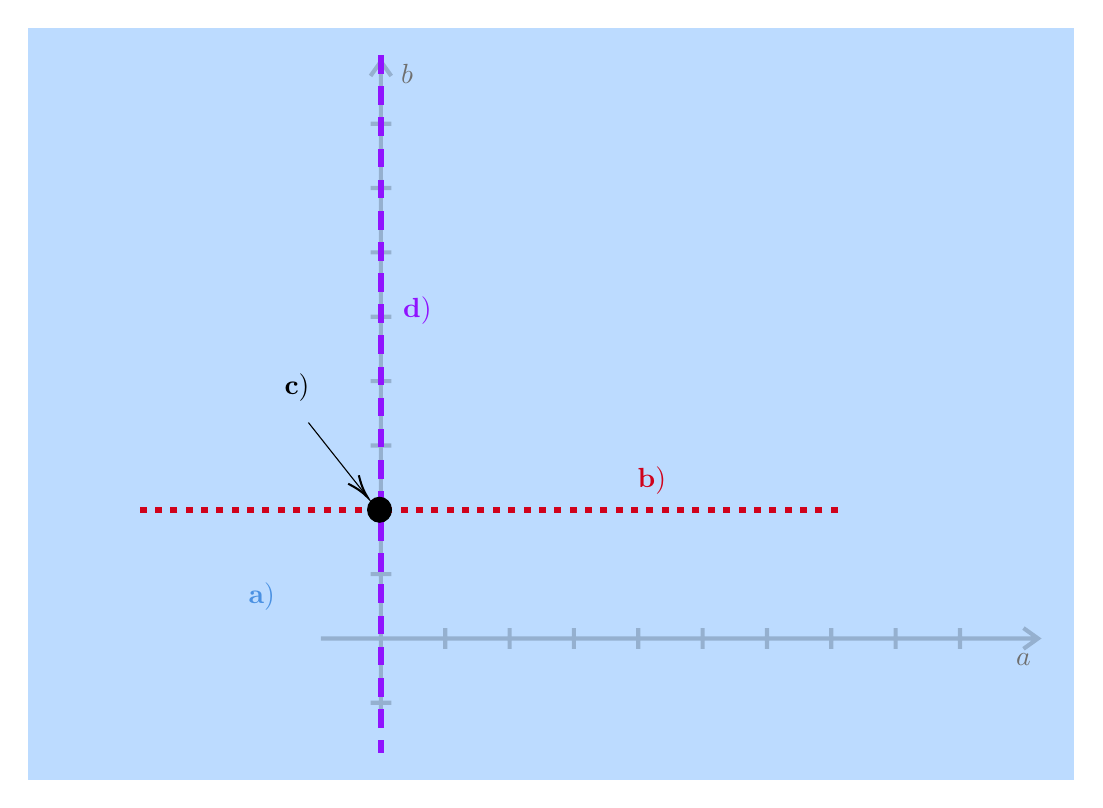
\begin{tikzpicture}[x=0.75pt,y=0.75pt,yscale=-1,xscale=1]
	%uncomment if require: \path (0,362); %set diagram left start at 0, and has height of 362

	%Shape: Rectangle [id:dp5897803105181249] 
	\draw  [color={rgb, 255:red, 0; green, 0; blue, 0 }  ,draw opacity=0 ][fill={rgb, 255:red, 46; green, 144; blue, 255 }  ,fill opacity=0.32 ] (101.5,-1) -- (605.5,-1) -- (605.5,361) -- (101.5,361) -- cycle ;
	%Shape: Axis 2D [id:dp9924581920490461] 
	\draw [color={rgb, 255:red, 91; green, 112; blue, 136 }  ,draw opacity=0.4 ][line width=1.5]  (242.5,293.01) -- (588,293.01)(271.41,15) -- (271.41,331) (581,288.01) -- (588,293.01) -- (581,298.01) (266.41,22) -- (271.41,15) -- (276.41,22) (302.41,288.01) -- (302.41,298.01)(333.41,288.01) -- (333.41,298.01)(364.41,288.01) -- (364.41,298.01)(395.41,288.01) -- (395.41,298.01)(426.41,288.01) -- (426.41,298.01)(457.41,288.01) -- (457.41,298.01)(488.41,288.01) -- (488.41,298.01)(519.41,288.01) -- (519.41,298.01)(550.41,288.01) -- (550.41,298.01)(266.41,262.01) -- (276.41,262.01)(266.41,231.01) -- (276.41,231.01)(266.41,200.01) -- (276.41,200.01)(266.41,169.01) -- (276.41,169.01)(266.41,138.01) -- (276.41,138.01)(266.41,107.01) -- (276.41,107.01)(266.41,76.01) -- (276.41,76.01)(266.41,45.01) -- (276.41,45.01)(266.41,324.01) -- (276.41,324.01) ;
	\draw   ;
	%Straight Lines [id:da6947499728767902] 
	\draw [color={rgb, 255:red, 144; green, 19; blue, 254 }  ,draw opacity=1 ][line width=2.25]  [dash pattern={on 6.75pt off 4.5pt}]  (271.41,11.99) -- (271.41,348.02) ;


	%Straight Lines [id:da6140862155635209] 
	\draw [color={rgb, 255:red, 208; green, 2; blue, 27 }  ,draw opacity=1 ][line width=2.25]  [dash pattern={on 2.53pt off 3.02pt}]  (491.5,231) -- (153.58,231) ;


	%Shape: Ellipse [id:dp5880814449962952] 
	\draw  [fill={rgb, 255:red, 0; green, 0; blue, 0 }  ,fill opacity=1 ] (265,231) .. controls (265,227.69) and (267.57,225) .. (270.75,225) .. controls (273.93,225) and (276.5,227.69) .. (276.5,231) .. controls (276.5,234.31) and (273.93,237) .. (270.75,237) .. controls (267.57,237) and (265,234.31) .. (265,231) -- cycle ;
	%Straight Lines [id:da609701303428703] 
	\draw    (236.5,189) -- (263.76,223.43) ;
	\draw [shift={(265,225)}, rotate = 231.63] [color={rgb, 255:red, 0; green, 0; blue, 0 }  ][line width=0.75]    (10.93,-3.29) .. controls (6.95,-1.4) and (3.31,-0.3) .. (0,0) .. controls (3.31,0.3) and (6.95,1.4) .. (10.93,3.29)   ;


	% Text Node
	% \draw (721,21) node   {$0$};
	% Text Node
	% \draw (701,71) node   {$0$};
	% Text Node
	\draw (214,273) node [color={rgb, 255:red, 74; green, 144; blue, 226 }  ,opacity=1 ]  {$\mathbf{a)}$};
	% Text Node
	\draw (231,172) node [color={rgb, 255:red, 0; green, 0; blue, 0 }  ,opacity=1 ]  {$\mathbf{c)}$};
	% Text Node
	\draw (402,217) node [color={rgb, 255:red, 208; green, 2; blue, 27 }  ,opacity=1 ]  {$\mathbf{b)}$};
	% Text Node
	\draw (289,135) node [color={rgb, 255:red, 144; green, 19; blue, 254 }  ,opacity=1 ]  {$\mathbf{d)}$};
	% Text Node
	\draw (581,303) node [color={rgb, 255:red, 111; green, 111; blue, 111 }  ,opacity=1 ]  {$a$};
	% Text Node
	\draw (284,21) node [color={rgb, 255:red, 111; green, 111; blue, 111 }  ,opacity=1 ]  {$b$};
\end{tikzpicture}
\end{center}
\end{solution}

\begin{problem}[System of linear equations; 6pt]
	\rm
	Write a system of linear equations consisting of $m$ equations in $n$ unknowns with 
	\begin{center}
		(a)~no solutions; \hfil
		(b)~exactly one solution; \hfil
		(c)~infinitely many solutions \\[5pt]
	\end{center}
	for (i) $m=n=3$; (ii) $m=3$ and $n=2$; (iii) $m=2$, $n=3$.
\end{problem}


\begin{solution}[]\rm
.\\
\begin{enumerate}[(i)]
\item
\[
(a)
\left\{\begin{matrix}
x_1 + 9x_2 + x_3 = 1 \\
9x_1 + 81x_2 + 9x_3 = 101 \\
8x_1 - 21x_2 + 14x_3 = 20 \\
\end{matrix}\right.
\quad (b)
\left\{\begin{matrix}
5x_1 + 3x_2 + 2x_3 = 1 \\
x_1 + 4x_2 + 3x_3 = 1 \\
2x_1 + 1x_2 + 1x_3 = 1 \\
\end{matrix}\right.
\quad (c)
\left\{\begin{matrix}
3x_1 - x_2 - 2x_3 = 5 \\
5x_1 + 12x_2 - 6x_3 = 23 \\
9x_1 - 3x_2 - 6x_3 = 15 \\
\end{matrix}\right.
\]
\item
\[
(a)
\left\{\begin{matrix}
2x_1 +  x_2 = 12 \\
 x_1 +  x_2 = 3 \\
3x_1 + 3x_2 = 1 \\
\end{matrix}\right.
\quad (b)
\left\{\begin{matrix}
2x_1 +  x_2 = 12 \\
 x_1 +  x_2 = 3 \\
3x_1 + 3x_2 = 9 \\
\end{matrix}\right.
\quad (c)
\left\{\begin{matrix}
x_1 - x_2 = 2 \\
-x_1 + x_2 = -2 \\
5x_1 - 5x_2 = 10 \\
\end{matrix}\right.
\]
\item
\[
(a)
\left\{\begin{matrix}
15x_1 + 5x_2 + 10x_3 = 25 \\
3x_1 + x_2 + 2x_3 = 10 \\
\end{matrix}\right.
\quad (b)
\begin{matrix}
\text{there is no such system,}\\
\text{not enough equations}\\
\text{for 3 unknowns.\qquad}\\
\text{(should be} \geq 3)~\qquad
\end{matrix}
\quad (c)
\left\{\begin{matrix}
x_1 - x_2 + x_3 = 5 \\
13x_1 + 4x_2 - 8x_3 = -9 \\
\end{matrix}\right.
\]
\end{enumerate}\end{solution}


\begin{problem}[System of linear equations; 4pt]\rm
	The following are coefficient matrices of linear systems. For each system, what can you say about the number of solutions to the corresponding system \textbf{(i)} in the homogeneous case (when $b_1 = \dots =b_m =0$) and \textbf{(ii)} for a generic RHS?
	\[
	\textrm{(a)}\begin{pmatrix}
		1 &   4 \\ 2 & 1
		\end{pmatrix},
	\qquad
	\textrm{(b)}\begin{pmatrix}
		1 &  4  & 3\\ 2 & 1 & 0
		\end{pmatrix},
	\qquad
	\textrm{(c)}\begin{pmatrix}
		2 & 1 \\ 1 &  4 \\ 0 & 3
		\end{pmatrix},
	\qquad
	\textrm{(d)}\begin{pmatrix}
		1 & 4 & 3 \\ 2 & 1 & 0 \\ 1 & 1 & 1
		\end{pmatrix}.
	\]
\end{problem}

\begin{solution}[]\rm Let $(A~|~b)$ denote the augmented matrix of linear system.
\begin{enumerate}[(a)]
\item
\[
\begin{pmatrix}
1 &   4 \\ 2 & 1
\end{pmatrix}
\sim
\begin{pmatrix}
1 &   4 \\ 0 & -7
\end{pmatrix}
\]
\begin{enumerate}[(i)]
\item $\rank(A)=2~\Rightarrow$ exactly one solution.
\item $\rank(A~|~b)=\rank(A)=2~\Rightarrow$ exactly one solution.
\end{enumerate}
\item
\[
\begin{pmatrix}
1 &  4  & 3\\ 2 & 1 & 0
\end{pmatrix}
\sim
\begin{pmatrix}
1 &  4  & 3\\ 0 & -7 & -6
\end{pmatrix}
\]
\begin{enumerate}[(i)]
\item $\rank(A)=2<3~\Rightarrow$ the infinite number of solutions.
\item $\rank(A~|~b)=\rank(A)=2<3~\Rightarrow$ the infinite number of solutions.
\end{enumerate}
\item
\[
\begin{pmatrix}
2 & 1 \\ 1 &  4 \\ 0 & 3
\end{pmatrix}
\sim
\begin{pmatrix}
1 & 4 \\ 0 &  -7 \\ 0 & 3
\end{pmatrix}
\]
\begin{enumerate}[(i)]
\item $\rank(A)=2~\Rightarrow$ exactly one solution.
\item $\rank(A)=2$; $\rank(A~|~b)$ may be $2$ or $3$, if $2~\Rightarrow$ exactly one solution, otherwise there is no solution.
\end{enumerate}
\item
\[
\begin{pmatrix}
1 & 4 & 3 \\ 2 & 1 & 0 \\ 1 & 1 & 1
\end{pmatrix}
\sim
\begin{pmatrix}
1 & 4 & 3 \\ 0 & -7 & -6 \\ 0 & -3 & -2
\end{pmatrix}
\sim
\begin{pmatrix}
1 & 4 & 3 \\ 0 & -7 & -6 \\ 0 & 0 & 4/7
\end{pmatrix}
\]
\begin{enumerate}[(i)]
\item $\rank(A)=3~\Rightarrow$ exactly one solution.
\item $\rank(A~|~b)=\rank(A)=3~\Rightarrow$ exactly one solution.\\
\end{enumerate}
\end{enumerate}
\end{solution}


\begin{problem}[System of linear equations; linear dependence; 3pt]\rm
	Prove that any $n+1$ vectors in $\bR^n$ are linearly dependent.
	
	\small{\textsf{Hint: regard a linear combination of these vectors resulting in a zero vector as a homogeneous linear system and show that it possesses a non-trivial solution}}
\end{problem}

\begin{solution}[]\rm Let $\{a_1 \dots a_{n+1}\}$ be the set of $n+1$ vectors in $\mathbb{R}^n$. If $\{a_1 \dots a_{n}\}$ is a linearly dependent set then $\{a_1 \dots a_{n+1}\}$ is also a linearly dependent set. Now consider $\{a_1 \dots a_{n}\}$ is a linearly independent set. We need to prove that there exist $x_1 \dots x_{n+1}$, not equal to $0$ simultaneously, such that
\[
\sum_1^{n+1}x_i a_i = 0
\]
If we denote
\[
A =
\begin{pmatrix} a_1 & \cdots & a_{n+1} \end{pmatrix} =
\begin{pmatrix}
a^1_1 & \cdots & a^1_n & a^1_{n+1} \\
\vdots & & \vdots & \vdots \\
a^n_1 & \cdots & a^n_n & a^n_{n+1}
\end{pmatrix} 
\qquad
x = \begin{pmatrix} x_1 & \cdots & x_{n+1} \end{pmatrix}^\top
\]
then we need to find a non-trivial solution of $Ax = 0$.
Since $\{a_1 \dots a_{n}\}$ is a linearly independent set $\Rightarrow \rank(A) = n$ (suppose that $a^1_1 \neq 0$):
\[
\Rightarrow
\begin{pmatrix}
a^1_1 & \cdots & a^1_{n} \\
\vdots & & \vdots \\
a^n_1 & \cdots & a^n_{n}
\end{pmatrix} 
\sim
\begin{pmatrix}
a^1_1 & a^1_2 & \cdots & a^1_n \\
0 & \hat a^2_2 & \cdots & \hat a^2_n \\
\vdots &  & \ddots & \vdots \\
0 & 0 & \cdots & \hat a^n_n
\end{pmatrix} \quad \text{and} \quad \hat a^k_k \neq 0 \quad \forall k=\overline{1,n}
\]
\[
\Rightarrow
A = \begin{pmatrix}
a^1_1 & \cdots & a^1_{n} & a^1_{n+1} \\
\vdots & & \vdots & \vdots \\
a^n_1 & \cdots & a^n_{n} & a^n_{n+1}
\end{pmatrix} 
\sim
\begin{pmatrix}
a^1_1 & a^1_2 & \cdots & a^1_n & a^1_{n+1} \\
0 & \hat a^2_2 & \cdots & \hat a^2_n & \hat a^2_{n+1} \\
\vdots &  & \ddots & \vdots & \vdots \\
0 & 0 & \cdots & \hat a^n_n & \hat a^n_{n+1}
\end{pmatrix}
\]
\[
\hat a^n_n x_n + \hat a^n_{n+1} x_{n+1} = 0
\]
If $\hat a^n_{n+1} = 0$ then $x_n = 0$ and $x_{n+1} \in \mathbb{R} \Rightarrow$ with $x_{n+1} \neq 0$ the non-trivial solution is found.\\
Otherwise $x_{n+1} = - \frac{\hat a^n_n}{\hat a^n_{n+1}} x_n $. We can substitute $x_{n+1}$ by this and get $n \times n-1$ system now. And so on analogically we can reach zero coefficient or remaining $x_1$ and $x_2$ and see that we may choose one of these values so we can get a non-trivial solution.
\\\end{solution}

\begin{problem}[Gauss elimination; determinants; 2pt]\rm 
	Determine all the values of~$k$ for which the column vectors below are linearly dependent:
	\begin{equation*}
	\mathrm{(a)}\quad
	\begin{pmatrix}[r]
	1 \\ 2 \\ -1
	\end{pmatrix},
	\begin{pmatrix}[r]
	2 \\ -3 \\ 5
	\end{pmatrix},
	\begin{pmatrix}[r]
	\,6\, \\ \,k\, \\ \,1\,
	\end{pmatrix};
	\qquad
	\mathrm{(b)}\quad \begin{pmatrix}[r]
	-1 \\ 2 \\1
	\end{pmatrix},
	\begin{pmatrix}[r]
	2 \\ -4 \\ -2
	\end{pmatrix},
	\begin{pmatrix}[r]
	\,k\, \\ \,3\, \\ -3\,
	\end{pmatrix}
	\end{equation*}
\end{problem}

\begin{solution}[]\rm Let A denote a matrix composed of given column vectors. Vectors are linearly dependent $~\Leftrightarrow~\det A = 0~\Leftrightarrow~\rank(A) < 3$.
\begin{enumerate}[(a)]
\item
\[
\begin{pmatrix}
1 & 2 & 6\\
2 & -3 & k\\
-1 & 5 & 1
\end{pmatrix}
\sim
\begin{pmatrix}
1 & 2 & 6\\
0 & -7 & k-24\\
0 & 7 & 7
\end{pmatrix}
\sim
\begin{pmatrix}
1 & 2 & 6\\
0 & 7 & 7 \\
0 & 0 & k-17\\
\end{pmatrix}
\Rightarrow k =17
\]
\item
\[
\begin{pmatrix}
-1 & 2 & k\\
2 & -4 & 3\\
1 & -2 & -3
\end{pmatrix}
\sim
\begin{pmatrix}
1 & -2 & -3\\
0 & 0 & 9\\
0 & 0 & k-3
\end{pmatrix}
\Rightarrow k \in \mathbb{R}
\]
\end{enumerate}
\end{solution}


\begin{problem}[Matrix algebra; 4pt]\rm 
	Let $\mathbf{0}_n$  and $I_n$ denote respectively the zero and identity matrices of size~$n$ (say, $n=10$).
	\begin{enumerate}[(a)]
		\item Is there an $n\times n$ matrix $A$ such that $A\ne\mathbf{0}_n$ and $A^2 = \mathbf{0}_n$? Justify your answer.
		\item Is there an $n\times n$ matrix $A$ such that $A\ne\mathbf{0}_n, I_n$ and $A^2 = A$? Justify your answer.
		\item Is there an $n\times n$ matrix $A$ such that $A\ne I_n$ and $A^2 = I_n$? Justify your answer.
		\item Are there $n\times n$ matrices $A$ and $B$ such that $A\ne \mathbf{0}_n$, $B\ne\mathbf{0}_n$, $AB \ne \mathbf{0}_n$ but $BA = \mathbf{0}_n$?
	\end{enumerate}

	
\small{\textsf{Hint: analyse the case $n=2$ to guess the answer and then try to see the pattern in higher dimensions}}
\end{problem}

\begin{solution}[]\rm \quad
	\begin{enumerate}[(a)]\rm
		\item Yes, e.g.:\\
		If $n \mod 2 = 0$ then:
		\[
		A = \begin{pmatrix}
		1 & -1 &\cdots & 1 & -1 \\ 
		1 & -1 &\cdots & 1 & -1  \\
		\vdots & \vdots &  & \vdots & \vdots \\
		1 & -1 &\cdots & 1 & -1  \\
		1 & -1 &\cdots & 1 & -1
		\end{pmatrix}
		\]
		(for $n=2$ we have $A = \begin{pmatrix}1 & -1 \\ 1 & -1\end{pmatrix}$ so $A^2 = \begin{pmatrix}1 & -1 \\ 1 & -1\end{pmatrix} \begin{pmatrix}1 & -1 \\ 1 & -1\end{pmatrix} = \begin{pmatrix}1-1 & 1-1 \\ -1+1 & -1+1\end{pmatrix} = \mathbf{0}_n$ etc.).\\[10pt]
		If $n \mod 2 \neq 0$ then:
		\[
		A = \begin{pmatrix}
		1 & -1 &\cdots & 1 & -1 & 0\\ 
		1 & -1 &\cdots & 1 & -1  & 0\\
		\vdots & \vdots & & \vdots & \vdots & \vdots \\
		1 & -1 &\cdots & 1 & -1 & 0 \\
		1 & -1 &\cdots & 1 & -1 & 0
		\end{pmatrix}
		\]
		(for $n=3$: $A = \begin{pmatrix}1 & -1 & 0\\ 1 & -1 & 0\\ 1 & -1 & 0\end{pmatrix}$ so $A^2 = \begin{pmatrix}1-1+0 & 1-1+0 & 1-1+0\\ -1+1+0 & -1+1+0 & -1+1+0\\ 0 & 0 & 0\end{pmatrix}=\mathbf{0}_n$ etc.).
		\item Yes, e.g. let $B$ be an $n\times n$ matrix such that $B^\top B$ is not singular. Then $B(B^\top B)^{-1}B^\top $ is idempotent:
		\[
		B(B^\top B)^{-1}(B^\top B)(B^\top B)^{-1}B^\top =B(B^\top B)^{-1}B^\top 
		\]
		Since we can find such B (e.g. $B=\begin{pmatrix}
		1 &\cdots & 0 & 0\\ 
		\vdots & \ddots & \vdots & \vdots \\
		0 &\cdots & 1 & 0  \\
		0 &\cdots & 0 & 5
		\end{pmatrix}$) then $A=B(B^\top B)^{-1}B^\top \neq I_n$, $\neq \mathbf{0}_n$.
		\item Yes, e.g.:
		\[
		A = \begin{pmatrix}
		0 & \cdots & 0 & 1 \\ 
		0 & \cdots & 1 & 0  \\
		\vdots & \reflectbox{$\ddots$} & \vdots & \vdots \\
		1 & \cdots & 0 & 0
		\end{pmatrix}
		\]
		So $A^2 = I_n$
		\item Yes, e.g.:\\
		\[
		A = \begin{pmatrix}
		1 & 1 &\cdots & 1 \\ 
		1 & 1 &\cdots & 1  \\
		\vdots & \vdots & \ddots  & \vdots \\
		1 & 1 &\cdots & 1
		\end{pmatrix} 
		\]
		and if $n \mod 2 = 0$ then:
		\[
		B = \begin{pmatrix}
		1 & -1 &\cdots & 1 & -1 \\ 
		1 & -1 &\cdots & 1 & -1  \\
		\vdots & \vdots &  & \vdots & \vdots \\
		1 & -1 &\cdots & 1 & -1  \\
		1 & -1 &\cdots & 1 & -1
		\end{pmatrix}
		\]
		otherwise:
		\[
		B = \begin{pmatrix}
		1 & -1 &\cdots & 1 & -1 & 0\\ 
		1 & -1 &\cdots & 1 & -1  & 0\\
		\vdots & \vdots &  & \vdots & \vdots & \vdots \\
		1 & -1 &\cdots & 1 & -1 & 0 \\
		1 & -1 &\cdots & 1 & -1 & 0
		\end{pmatrix}
		\]
		One can see that $BA=\mathbf{0}_n$ and that $AB \neq \mathbf{0}_n$ (the element $(AB)_{11}$ is already equal to $ n \neq 0$)
	\end{enumerate}
\end{solution}

\begin{problem}[Determinants and cross-products; 4pt]\rm \rm
	A parallelepiped has edges from $(0;0;0)$ to $(2;1;1)$, $(1;2;1)$, and $(1;1;2)$. Find its volume and also find the area of each parallelogram face.
	
    \small{\textsf{Hint: a cross-, or vector-product in $\bR^3$ is handy here. Also, recall the geometric meaning of determinant}}
\end{problem}

\begin{solution}[]\rm \quad \\
Volume:
\[
V = \left | a \cdot (b \times c)\right | = \left| \det
\begin{pmatrix}
a_1 & a_2 & a_3 \\
b_1 & b_2 & b_3 \\
c_1 & c_2 & c_3 \\
\end{pmatrix}
 \right| = \left| \det
\begin{pmatrix}
2 & 1 & 1 \\
1 & 2 & 1 \\
1 & 1 & 2 \\ 
\end{pmatrix}
 \right| = \left| 8 + 1 + 1 - 2 - 2 - 2 \right|  = 4
\]\\
Area of parallelograms based on $ab$, $bc$ and $ac$:
\[
S_{ab} = \left| \det  
\begin{pmatrix}
i & j & k \\
a_1 & a_2 & a_3 \\
b_1 & b_2 & b_3 \\
\end{pmatrix}
\right| = \left| \det  
\begin{pmatrix}
i & j & k \\
2 & 1 & 1 \\
1 & 2 & 1 \\
\end{pmatrix}
\right|
= \left| \det 
\begin{pmatrix}
1 & 1 \\
2 & 1 \\
\end{pmatrix} i - \det 
\begin{pmatrix}
2 & 1 \\
1 & 1 \\
\end{pmatrix} j + \det 
\begin{pmatrix}
2 & 1 \\
1 & 2 \\
\end{pmatrix} k
 \right| = \]\[=\left| (-1,-1,3)^\top \right| = \sqrt{1+1+9} = \sqrt{11}
\]\\
\[
S_{bc} = \left| \det 
\begin{pmatrix}
i & j & k \\
b_1 & b_2 & b_3 \\
c_1 & c_2 & c_3 \\
\end{pmatrix}
\right| = \left| \det 
\begin{pmatrix}
i & j & k \\
1 & 2 & 1 \\
1 & 1 & 2 \\ 
\end{pmatrix}
\right|
= \left| \det 
\begin{pmatrix}
2 & 1 \\
1 & 2 \\
\end{pmatrix} i - \det 
\begin{pmatrix}
1 & 1 \\
1 & 2 \\
\end{pmatrix} j + \det 
\begin{pmatrix}
1 & 2 \\
1 & 1 \\
\end{pmatrix} k
 \right| = \]\[=\left| (3,-1,-1)^\top \right| = \sqrt{11}
\]\\
\[
S_{ac} = \left| \det 
\begin{pmatrix}
i & j & k \\
b_1 & b_2 & b_3 \\
c_1 & c_2 & c_3 \\
\end{pmatrix}
\right| = \left| \det 
\begin{pmatrix}
i & j & k \\
2 & 1 & 1 \\
1 & 1 & 2 \\  
\end{pmatrix}
\right|
= \left| \det 
\begin{pmatrix}
1 & 1 \\
1 & 2 \\
\end{pmatrix} i - \det 
\begin{pmatrix}
2 & 1 \\
1 & 2 \\
\end{pmatrix} j + \det 
\begin{pmatrix}
2 & 1 \\
1 & 1 \\
\end{pmatrix} k
 \right| = \]\[=\left| (1,-3,1)^\top \right| = \sqrt{11}
\]
\\\end{solution}

\begin{problem}[Determinants and matrix algebra; 2pt]\rm
	Assume that $3 \times 3$ matrices $A$, $B$ and $C$ are as follows
	\[
	A = \begin{pmatrix}\textrm{row~1} \\  \textrm{row~2} \\  \textrm{row~3}\end{pmatrix}
	\qquad
	B = \begin{pmatrix}
	\textrm{row~1 + row 2} \\  \textrm{row~2 + row 3} \\  \textrm{row~3 + row 1}
	\end{pmatrix}
	\qquad
	C = \begin{pmatrix}
	\textrm{row~1 $-$ row 2} \\  \textrm{row~2 $-$ row 3}
	\\  \textrm{row~3 $-$ row 1}
	\end{pmatrix}
	\]
	Given that $\det(A) = 5$, find $\det(B)$ and $\det(C)$.
	
	    \small{\textsf{Hint: use the elementary row operations to produce $B$ from $A$; an alternative (and more elegant) way is to find a matrix $B'$ such that $B=B'A$; the same for $C$}}
\end{problem}

\begin{solution}[]\rm
\[
B = 
\begin{pmatrix}
1 & 1 & 0 \\
0 & 1 & 1 \\
1 & 0 & 1 \\
\end{pmatrix} \begin{pmatrix}\textrm{row~1} \\  \textrm{row~2} \\  \textrm{row~3}\end{pmatrix} = B'A \Rightarrow
B' = 
\begin{pmatrix}
1 & 1 & 0 \\
0 & 1 & 1 \\
1 & 0 & 1 \\
\end{pmatrix}
\]
Hence
\[
\det B = \det (B'A) = \det B' \det A = (1 + 1 + 0) \det A  = 10
\]\\[1pt]
\[
C = 
\begin{pmatrix}
1 & -1 & 0 \\
0 & 1 & -1 \\
-1 & 0 & 1 \\
\end{pmatrix} \begin{pmatrix}\textrm{row~1} \\  \textrm{row~2} \\  \textrm{row~3}\end{pmatrix} = C'A
\Rightarrow
C' = 
\begin{pmatrix}
1 & -1 & 0 \\
0 & 1 & -1 \\
-1 & 0 & 1 \\
\end{pmatrix}
\]
Hence
\[
\det C = \det (C'A) = \det C' \det A = (1 - 1 + 0) \det A  = 0
\]
\\\end{solution}

\begin{problem}[Determinants; eigenvalues and their properties; 3pt]\rm
	Using any of the methods, find all $\lambda$ for which the matrix below is singular:
	\[
	A - \lambda I = \begin{pmatrix}
	a -\lambda & b & c & d \\  a & b-\lambda & c & d  
	\\ a & b & c-\lambda & d \\ a & b & c & d-\lambda
	\end{pmatrix}
	\]
	
	 \small{\textsf{Hint: one approach is to calculate the determinant and find its roots. An alternative approach is to identify the $\lambda$'s looked for as eigenvalues of~$A$. Note $A$ is of rank $1$; what conclusions on eigenvalues can you derive? }}
\end{problem}

\begin{solution}[]\rm
One can see that:
\[
	A = \begin{pmatrix}
	a  & b & c & d \\  a & b & c & d  
	\\ a & b & c & d \\ a & b & c & d
	\end{pmatrix}
\]
$A - \lambda I$ is singular $\Leftrightarrow det(A - \lambda I) = 0 \Leftrightarrow Av = \lambda v$ has a non-zero solution w.r.t $v$.
\[  \Rightarrow
av_1 + bv_2 + cv_3 + dv_4 = \lambda v_1 = \lambda v_2 = \lambda v_3 = \lambda v_4 \neq 0
\]
\[  \Rightarrow
\left\{\begin{matrix}
v_1 = v_2 = v_3 = v_4 \neq 0  \\ 
(a + b + c + d)v_1 = \lambda v_1 
\end{matrix}\right.
 \]
\[  \Rightarrow
 \lambda = a + b + c + d
\]
\\\end{solution}


\begin{problem}[Rank of a matrix; 4pt] \rm \begin{enumerate}[(a)]
		\item Assume that $A$ and $B$ are matrices such that $AB$ is well defined. By comparing the column spaces of $A$ and $AB$, show that $\rank(AB)\le\rank(A)$. Transpose to conclude that also $\rank(AB)\le\rank(B)$.
		\item Assume that $A$ and $B$ are non-square matrices such that both $AB$ and $BA$ exist. Show that at least one of $AB$ or $BA$ is singular. 
	\end{enumerate}
	\small{\textsf{Hint: in (b), show that at least one of $AB$ and $BA$ is not of full rank}}
\end{problem}	

\begin{solution}[]\rm
\begin{enumerate}[(a)]
\item
Let A be a $n\times m$ matrix and $B$ -- a $m\times k$ matrix, so $AB$ is $n\times k$ matrix. We can rewrite matrices in the form of column-vectors:
\[
A = \begin{pmatrix} a_1 & \dots & a_m\end{pmatrix}
\quad
B = \begin{pmatrix} b_1 & \dots & b_k\end{pmatrix}
~\Rightarrow~
AB = \begin{pmatrix} Ab_1 & \dots & Ab_k\end{pmatrix}
\]
\[
\rank(AB) = \dim Im (AB) = \dim span \{Ab_1 \dots Ab_k\} \leq^*  \dim span \{a_1 \dots a_m\} = \dim Im (A) = rank (A)
\]
Below is shown that $^*$ is satisfied:
\[
\forall y \in Im (AB) = span \{Ab_1 \dots Ab_k\}~\exists x \in \mathbb{R}^k:~y = ABx = A(Bx)~\left(\exists Bx=z \in \mathbb{R}^m\right)
\]
\[
\Rightarrow y \in Im (A) = span \{a_1 \dots a_m\}
\]
Hence
\[
Im (AB) \subset Im(A) ~\Rightarrow~\dim Im (AB) \leq \dim Im(A)
\]\\[5pt]
\[
\rank(AB) = \rank(AB)^\top =\rank(B^\top A^\top) \leq \rank(B^\top) = \rank(B)
\]\\[5pt]
So
\[
\rank(AB) \leq \min\{\rank(A), \rank(B)\}
\]
\item Both existing $AB$ and $BA$ means that if $A$ is a $n\times m$ matrix then $B$ is a $m\times n$ matrix. Let $n<m$. $BA$ is a $m\times m$ matrix. And
\[
\rank(BA) \leq \min\{\rank(B), \rank(A)\} \leq n<m~\Rightarrow~\det(BA) = 0
\]
Hence $BA$ is singular.\\
And vice versa, if $m<n$ then $AB$ is singular.
\\
\end{enumerate}
\end{solution}


\begin{problem}[Trace of a matrix; 2pt]\rm
	Are there $n\times n$ matrices $A$ and $B$ such that $AB-BA = I_n$? 
\end{problem}	


\begin{solution}[]\rm
No, since $\left(AB-BA = I_n \right)\Rightarrow \left(\trace(AB-BA) = \trace(I_n)\right)$ one can show that the necessary condition isn't satisfied: \\
$
\trace(AB-BA)=\trace(AB)-\trace(BA)=\trace(AB)-\trace(AB)=0
$
, but:
$
\trace(I_n)=n \neq 0
$
\\\end{solution}


\begin{problem}[Bases; 3pt]\rm
	For what numbers $c$ are the following sets of vectors bases for $\bR^3$?
	\begin{itemize}
		\item[(a)] $(c,1,1)^\top$, $(1,-1,2)^\top$, $(3,4,-1)^\top$;
		\item[(b)] $(c,1,1)^\top$, $(1,-1,2)^\top$, $(-2,2,-4)^\top$;
		\item[(c)] $(c,1,1)^\top$, $(1,1,0)^\top$, $(0,1,2)^\top$, $(3,0,-1)^\top$;
		\item[(d)] $(c,1,1)^\top$, $(1,0,1)^\top$
	\end{itemize}
\end{problem}

\begin{solution}[]\rm .\\
Basis of $\bR^3$ is a set of 3 linearly independent vectors.
\begin{enumerate}[(a)]
\item The set should be linearly independent so we have a linear system:
\[
\begin{pmatrix}
c  & 1 & 3 \\
1  & -1 & 4 \\
1  & 2 & -1 \\
\end{pmatrix}
\sim
\begin{pmatrix}
1  & 2 & -1 \\
0  & 3 & -5 \\
0  & 1-2c & 3+c \\
\end{pmatrix}
\sim
\begin{pmatrix}
1  & 2 & -1 \\
0  & 3 & -5 \\
0  & 0 & 14-7c \\
\end{pmatrix}
\]
\[
~\Rightarrow ~14 - 7c \neq 0 ~\Rightarrow~ c \neq 2
\]
\item One can notice that $(1,-1,2)^\top$ and $(-2,2,-4)^\top$ are linearly dependent therefore the vectors in the whole set are linearly dependent so it already can't be a basis. Hence there is no proper number: $c \in  \varnothing $.
\item The number of vectors in the set is $4 \neq 3$, so it can't be a basis for any value of $c$. Hence $c \in \varnothing$
\item Same, the number of vectors in the set is $2 \neq 3$, so it can't be a basis for any value of $c$. Hence $c \in \varnothing$
\end{enumerate}
\end{solution}

\begin{problem}[Bases; transition matrices; 4pt]\rm
	Consider the bases $B = \{\bv_1,\bv_2,\bv_3\}$ and $B' = \{\bv'_1,\bv_2',\bv_3'\}$ for $\bR^3$, where
	\begin{alignat*}{3}
	\bv_1 &= \begin{pmatrix}[r] -3 \\ 0 \\ -3  \end{pmatrix},
	\qquad
	\bv_2 &= \begin{pmatrix}[r] -3 \\ 2 \\ -1  \end{pmatrix},
	\qquad
	\bv_3 &= \begin{pmatrix}[r] 1 \\ 6 \\ -1  \end{pmatrix}
	\\
	\bv_1' &= \begin{pmatrix}[r] -6 \\ -6 \\ 0  \end{pmatrix},
	\qquad
	\bv_2' &= \begin{pmatrix}[r] -2 \\ -6 \\ 4  \end{pmatrix},
	\qquad
	\bv_3' &= \begin{pmatrix}[r] -2 \\ -3 \\ 7  \end{pmatrix}
	\end{alignat*}
	\begin{enumerate}[(a)]
		\item Find the transition matrix $P_{B \to B'}$ from $B$ to $B'$.
		\item Compute the coordinate vector $(\bu)_B$ for $\bu = (-5,8,-5)^\top$.
		\item Use the transition matrix $P_{B \to B'}$ to compute the coordinate vector~$(\bu)_{B'}$.
		\item Check your work by computing $(\bu)_{B'}$ directly.
	\end{enumerate}
\end{problem}

\begin{solution}[]\rm
Given the bases of $B$ and $B'$ we can construct the transition matrices from each to $R = \{e_1, e_2, e_3\}$.
\[
P_{B \to R} = 
\begin{pmatrix}
-3 & -3 &  1 \\
0  &  2 &  6 \\
-3 & -1 & -1 \\
\end{pmatrix}
\qquad
P_{B' \to R} = 
\begin{pmatrix}
-6 & -2 & -2 \\
-6 & -6 & -3 \\
 0 &  4 &  7 \\
\end{pmatrix}
\]
\begin{enumerate}[(a)]
\item 
$P_{B \to B'} = P_{R \to B'} P_{B \to R} = P_{B' \to R}^{-1} P_{B \to R}$. We have to find the $P_{B' \to R}^{-1}$:
\[
\det P_{B' \to R} = 252+48-72 - 84 = 144
\]
\[
P_{B' \to R}^{-1} = \frac{1}{144}
\begin{pmatrix}
-30 &  42 & -24 \\
6   & -42 &  24 \\
-6  &  -6 &  24 \\
\end{pmatrix}^\top = \frac{1}{24}
\begin{pmatrix}
-5 &  1 & -1 \\
7  & -7 &  -1 \\
-4  &  4 &  4 \\
\end{pmatrix}
\]
Now we can compute $P_{B \to B'}$:
\[
P_{B \to B'} =  \frac{1}{24}
\begin{pmatrix}
-5 &  1 & -1 \\
7  & -7 &  -1 \\
-4  &  4 &  4 \\
\end{pmatrix}
\begin{pmatrix}
-3 & -3 &  1 \\
0  &  2 &  6 \\
-3 & -1 & -1 \\
\end{pmatrix}
= \frac{1}{12}
\begin{pmatrix}
 9 &  9  &   1 \\
-9 & -17 & -17 \\
 0 &  8  &  8 \\
\end{pmatrix}
\]
\item
$(\bu)_B = P_{R \to B} \bu = P_{B \to R}^{-1} \bu$. We have to find the $P_{B \to R}^{-1}$:
\[
\det P_{B \to R} = 6+54+6-18=48
\]
\[
P_{B \to R}^{-1} = \frac{1}{48}
\begin{pmatrix}
 4 & -18 &  6 \\
-4 &   6 &  6 \\
-20 & 18 & -6 \\
\end{pmatrix}^\top = \frac{1}{24}
\begin{pmatrix}
 2 & -2 & -10 \\
-9 &  3 & 9 \\
 3 &  3 & -3 \\
\end{pmatrix}
\]
Hence
\[
(\bu)_B = \frac{1}{24}
\begin{pmatrix}
 2 & -2 & -10 \\
-9 &  3 & 9 \\
 3 &  3 & -3 \\
\end{pmatrix}
\begin{pmatrix}-5\\8\\-5\\\end{pmatrix} = \frac{1}{24}
\begin{pmatrix}24\\24\\24\\\end{pmatrix} = \begin{pmatrix}1\\1\\1\\\end{pmatrix} 
\]
\item
\[
(\bu)_{B'} = P_{B \to B'} (\bu)_B = \frac{1}{12}
\begin{pmatrix}
 9 &  9  &   1 \\
-9 & -17 & -17 \\
 0 &  8  &  8 \\
\end{pmatrix} \begin{pmatrix}1\\1\\1\\\end{pmatrix} = \frac{1}{12}
\begin{pmatrix} 19 \\ -43 \\ 16 \\ \end{pmatrix} 
\]
\item
\[
(\bu)_{B'} = P_{R \to B'} \bu = 
P_{B' \to R}^{-1} \bu =  \frac{1}{24}
\begin{pmatrix}
-5 &  1 & -1 \\
7  & -7 &  -1 \\
-4  &  4 &  4 \\
\end{pmatrix}
\begin{pmatrix}-5\\8\\-5\\\end{pmatrix} = \frac{1}{24}
\begin{pmatrix}38\\-86\\32\\\end{pmatrix} = \frac{1}{12}
\begin{pmatrix}19\\-43\\16\\\end{pmatrix} 
\]
which matches the previous one.
\end{enumerate}
\end{solution}

\begin{problem}[Linear transformations; 2pt]\rm
	\begin{enumerate}[(a)]
		\item For what real values of parameters $a$ and $b$ there is a linear transformation of the space~$\mathbb{R}^3$ sending the vectors $\bu_1 = (1,0,0)^\top,\bu_2 = (1,a,0)^\top$, and $\bu_3 = (0,1,b)^\top$ into the vectors $\bv_1 = (0,0,1)^\top, \bv_2 = (0,b,1)^\top$, and $\bv_3 = (a,1,0)^\top$ respectively?
		\item For what $a$ and $b$ such a transformation is unique?
		\item For what $a$ and $b$ there exists an orthogonal transformation with this property?
	\end{enumerate}

	 \small{\textsf{Hint: yes, that's the problem from your entrance exam. However, nobody solved it correctly, and now you have a second chance!}}
\end{problem}



\begin{solution}[]\rm Let $u = \{\bu_1, \bu_2, \bu_3\}$ and $v = \{\bv_1, \bv_2, \bv_3\}$. Since we are dealing with $\mathbb{R}^3$ we need $\bu_i \neq \bu_j \quad \forall i\neq j$ and $ \bv_i \neq \bv_j \quad \forall i\neq j $ to have a unique transformation. Otherwise if some vectors match (which means that we have less than 3 unique vectors in $u$ or $v$) e.g. $\bu_1 = \bu_2$ then there exists a linear transformation only if the corresponding vectors $\bv_1 = \bv_2$ also match and then the transformation is not unique. Otherwise we have $A\bu_1 = \bv_1$ and $A\bu_2 = \bv_2$ so $A\bu_1 = A\bu_2 = \bv_2 \neq \bv_1$ which is impossible.\\
\begin{enumerate}[(a)]
\item In addition to finding such $a$, $b$ that there is a unique transformation (which is described below), we have to find such $a$, $b$ that $card(u) = card(v) < 3$ and matching vectors in $u$ correspond to the same matching vectors in $v$. One can see that $a = 0$ leads to $\bu_1 = \bu_2$, hence $\bv_1 = \bv_2$ that forces $b=0$. If $a = 0 \wedge b \neq 0$ then (as described above) a contradiction arises, the same with $a \neq 0 \wedge b = 0$. So the answer is $(a,b) \in \{(0,0)\} \cup \{(a,b) \in \mathbb{R}^2~\vline~a \neq 0 \wedge b \neq 0\} $.
Indeed, we have
\[
\bu_1 = \bu_2 = (1,0,0)^\top \quad
\bu_3 = (0,1,0)^\top \quad
\bv_1 = \bv_2 = (0,0,1)^\top \quad
\bv_3 = (0,1,0)^\top
\]
\[
A\begin{pmatrix}1\\0\\0\\\end{pmatrix} = \begin{pmatrix}0\\0\\1\\\end{pmatrix} \Rightarrow column_1(A) = \begin{pmatrix}0\\0\\1\\\end{pmatrix}
\]
\[
A\begin{pmatrix}0\\1\\0\\\end{pmatrix} = \begin{pmatrix}0\\1\\0\\\end{pmatrix} \Rightarrow column_2(A) = \begin{pmatrix}0\\1\\0\\\end{pmatrix}
\]
Hence
\[
A = \begin{pmatrix}
0 & 0 & a_1\\
0 & 1 & a_2\\
1 & 0 & a_3\\
\end{pmatrix} \quad a_i \in \mathbb{R} \quad i=\overline{1,3}
\]
\item So, for the unique transformation we need to have 3 unique vectors in $u$ and 3 unique vectors in $v$ which is equivalent to $a \neq 0 \wedge b \neq 0$. To make sure we'll find this linear transformation A. The transition scheme:\\

\begin{center}
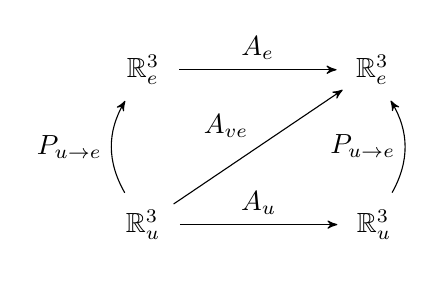
\begin{tikzpicture}[node distance=2cm and 2cm,>=stealth',auto, every place/.style={draw}]
    \node [place] (S1) {$\mathbb{R}_e^3$};
    \coordinate[node distance=1cm,left of=S1] (left-S1);
    \coordinate[node distance=0cm,right of=S1] (right-S1);
    \node [place] (S2) [right=of S1] {$\mathbb{R}_e^3$};
    \node [place] (S3) [node distance=1.5cm,below =of right-S1] {$\mathbb{R}_u^3$};    
    \node [place] (S4) [right=of S3] {$\mathbb{R}_u^3$};
    \path[->] (S1) edge  node {$A_e$} (S2);
    \path[->] (S3) edge [bend left] node {$P_{u \to e}$} (S1);
    \path[->] (S4) edge [bend right] node {$P_{u \to e}$} (S2);
    \path[->] (S3) edge  node {$A_u$} (S4);
    \path[->] (S3) edge  node {$A_{ve}$} (S2);      
\end{tikzpicture}
\end{center}

\[
P_{u \to e} = 
\begin{pmatrix}
1 &  1 & 0 \\
0  & a & 1 \\
0  & 0 & b \\
\end{pmatrix} \qquad
A_{ve} = 
\begin{pmatrix}
0 &  0 & a \\
0  & b & 1 \\
1  & 1 & 0 \\
\end{pmatrix}
\]
We need to find $A = A_e$:
\[
A_e = A_{ve} P_{e \to u} = A_{ve} P_{u \to e}^{-1}
\]
\[
\det P_{u \to e} = ab \qquad
P_{u \to e}^{-1} = \frac{1}{ab}
\begin{pmatrix}
ab & -b &  1 \\
0  &  b & -1 \\
0  &  0 &  a \\
\end{pmatrix}
\]
\[
\Rightarrow
A_e = \frac{1}{ab}
\begin{pmatrix}
0 &  0 & a \\
0  & b & 1 \\
1  & 1 & 0 \\
\end{pmatrix}
\begin{pmatrix}
ab & -b &  1 \\
0  &  b & -1 \\
0  &  0 &  a \\
\end{pmatrix} = \frac{1}{ab}
\begin{pmatrix}
0 &  0 & a^2 \\
0  & b^2 & a-b \\
ab  & 0 & 0 \\
\end{pmatrix} = 
\begin{pmatrix}
0 &  0 & \frac{a}{b} \\
0  & \frac{b}{a} & \frac{a-b}{ab} \\
1  & 0 & 0 \\
\end{pmatrix} 
\]
One can see that indeed $\forall i=\overline{1,3} \quad A_e \bu_i = \bv_i $. So the answer is $a \neq 0 \wedge b \neq 0$.\\[5pt]
\item $A$ is orthogonal when $A^\top = A^{-1}$. First let's check for a unique linear transformation when $a \neq 0 \wedge b \neq 0$:
\[
A^\top = \begin{pmatrix}
0 &  0 & 1 \\
0  & \frac{b}{a} & 0 \\
\frac{a}{b}  & \frac{a-b}{ab} & 0 \\
\end{pmatrix} 
\]
\[
\det A = -1 \qquad A^{-1} = - \begin{pmatrix}
 0 &  -\frac{b-a}{ab} & -\frac{b}{a} \\
 0  & -\frac{a}{b}    & 0 \\
-1  &  0              & 0 \\
\end{pmatrix}^\top = \begin{pmatrix}
0 &  0 & 1 \\
\frac{b-a}{ab}  & \frac{a}{b} & 0 \\
\frac{b}{a}  & 0 & 0 \\
\end{pmatrix} 
\]
Hence $a = b \Rightarrow A^\top = A^{-1}$. \\
Second, let's check for a non-unique linear transformation when $a = b = 0$:
\[
A^\top = \begin{pmatrix}
0 & 0 & 1\\
0 & 1 & 0\\
a_1 & a_2 & a_3\\
\end{pmatrix}
\]
\[
\det A = -a_1 \qquad  A^{-1} = \frac{1}{-a_1} \begin{pmatrix}
a_3 & a_2 & -1\\
0 & -a_1 & 0\\
-a_1 & 0 & 0\\
\end{pmatrix}^\top = \begin{pmatrix}
-\frac{a_3}{a_1} & 0 & 1\\
-\frac{a_2}{a_1} & 1 & 0\\
 \frac{1}{a_1}   & 0 & 0\\
\end{pmatrix}^\top
\]
\[
\Rightarrow 
\left\{\begin{matrix}
a_3 = 0 \\ 
a_2 = 0 \\
a_1 = \frac{1}{a_1}
\end{matrix}\right.
\Leftrightarrow 
\left\{\begin{matrix}
a_1 = \pm 1 \\
a_3 = 0 \\ 
a_2 = 0 \\
\end{matrix}\right.
\]
Hence for $a = b = 0$ there exists such orthogonal transformation. \\
So the answer is $(a,b) \in \{(a,a)~\vline~a \in\mathbb{R}\}$.
\end{enumerate}
\end{solution}

\vspace{1cm}

% % \begin{center}
% % 	\Large\bf{Linear Algebra\\
% % 		Homework 1: Bonus problem}
% % \end{center}

% % %\vspace{.5cm}


% % \begin{problem}[extra 5\%]\rm
% % 	Undergraduate students like linear systems whose coefficient matrices have integer entries and whose determinant is $\pm1$ (do you see why?). 
% % 	\begin{enumerate}[(a)]
% % 		\item Suggest a method generating all $3\times 3$ matrices of this type with relatively small entries (e.g. at most $100$ in absolute value). How can one easily find the inverse of such a matrix? Think of efficiency of your algorithm (e.g. as compared to the brute force approach); what is its complexity?
% % 		\item Suggest a method generating all $3\times 3$ matrices with integer entries between $-100$ and $100$ having pairwise orthogonal columns (no restriction on the determinant this time!).
% % 	\end{enumerate}
	

% % \end{problem}	

% % \textcolor{red}{
% % \begin{solution}[]\rm
% % \[
% % det \begin{pmatrix}
% % a_1 & a_2 & a_3 \\ 
% % b_1 & b_2 & b_3 \\
% % c_1 & c_2 & c_3
% % \end{pmatrix} = a_1 (b_2 c_3 - b_3 c_2) + a_2 (b_3 c_1 - b_1 c_3) + a_3 (b_1 c_2 - b_2 c_1)  = 1
% % \]
% % \end{solution}
% % }
\end{document}

